% Change to use the correct class file for your paper.
\documentclass{sig-alternate-10pt}

%\pagenumbering{arabic}

\usepackage{amsfonts}     % Adds math fonts, commands such as \begin{align}
\usepackage{array}        % Tables for use in math mode
\usepackage{booktabs}     % Elegant table-formatting library
\usepackage{bold-extra}   % Provides bf+sc (only in textbf+textsc env.)
\usepackage{bytefield}    % Formatting and layout of packets / bytefields
\usepackage[skip=5pt]{caption}
\usepackage{color}        % Allow the use and definition of colors
\usepackage{colortbl}     % Color table cells
\usepackage{comment}      % Provides \begin,\end{comment} for large blocks
%% \usepackage{cprotect}     % Allows verbatim, other formatting in macro args
\usepackage{endnotes}     % Footnotes pushed to the end of a document
\usepackage{gensymb}      % Adds useful symbols w/out math mode, e.g. \degree
\usepackage{graphicx}     % For importing graphics
\usepackage{hyperref}     % Creates hyperlinks from ref/cite 
\hypersetup{pdfstartview=FitH}
\usepackage{listings}     % in-line source code (poorly, consider minted)
\usepackage{mathtools}    % amsmath extension, adds more math formatting
\usepackage{multirow}     % Multiple row spacing in tables
\usepackage{nth}          % Typeset 33rd correctly as \nth{33}
%\usepackage[section]{placeins} % Don't let figs escape their sections
\usepackage{rotating}     % Rotates any object, note sideways != sidewaysfigure
%\usepackage[all=normal]{savetrees} % For when space is tight, read manual and
                          % selectively enable things. CAN BREAK CONF STYLES!!
\usepackage{soul}         % Provides \hl{} for highlighting
%\usepackage{subfig}
%\usepackage{subfigure}    % Complicated figure creation
%% \usepackage{subcaption}   % Replaces both subfig and subfigure
\usepackage[nofancy]{svninfo} % svn information in docs (req. svn:keywords)
\usepackage{tabularx}     % Complicated table creation
\usepackage{threeparttable} % Add footnotes to a table
\usepackage{units}        % For nice fractions, \nicefrac{1}{2} --> 1/2
\usepackage{url}          % Pretty printing of hyperlinks
\usepackage{xspace}       % Intelligently add spaces after commands

%% \DeclareCaptionType{copyrightbox}

\newlength\SUBSIZE

\renewcommand{\arraystretch}{1.2} % Space out rows in tables

%\setlength\paperheight {11in}
%\setlength\paperwidth {8.5in}

% Set the graphics path
\graphicspath{{../figs/}{../images/build/}}

% No space between bibliography items:
\let\oldthebibliography=\thebibliography
  \let\endoldthebibliography=\endthebibliography
  \renewenvironment{thebibliography}[1]{%
    \begin{oldthebibliography}{#1}%
      \setlength{\parskip}{0ex}%
      \setlength{\itemsep}{0ex}%
  }%
  {%
    \end{oldthebibliography}%
  }
\setlength{\parindent}{5mm}

\begin{document}

\title{FireDrill: Interactive DNS Rebinding}

% AUTHOR STYLE 1
\author{
 \alignauthor{Ryan Resig, Yunxing Dai}\\
 \affaddr{Electrical Engineering and Computer Science Department}\\
 \affaddr{University of Michigan}\\
 \affaddr{Ann Arbor, MI 48109}\\
 \email{\{rresig,yunxing\}@umich.edu}
}

% AUTHOR STYLE 2
\begin{comment}
\author{
\begin{tabular}{cc}
  \multicolumn{2}{c}{Author 1$^\dagger$, Author 2$^\dagger$, Author 3$^\dagger$, Author 4$^\ddagger$, and Author 5$^\dagger$\vspace{0.3cm}} \\
  \affaddr{$^\dagger$Computer Science \& Engineering Division} & \affaddr{$^\ddagger$Electrical and Computer Engineering Dept} \\ 
  \affaddr{University of Michigan} & \affaddr{Diff School}\\
  \affaddr{Ann Arbor, MI 48109} & \affaddr{Diff Address}\\
  \affaddr{\{u1,u2,u3,u4\}@eecs.umich.edu} & \affaddr{diffemail@email.com} \\
\end{tabular}
}
\end{comment}


\conferenceinfo{EECS 582 -- Winter'13} {Jan 10--Apr 23, 2013, Ann Arbor, Michigan, USA.}
\CopyrightYear{2013}
\crdata{XXX-X-XXXXX-XXX-X}

\maketitle

\begin{abstract}
% ABSTRACT
By using traditional DNS rebinding attacks, an attacker is able to circumvent firewalls in order to access internal network servers. Although many of the variations of this attack are well-known and sufficiently defended against, we show that by exploiting browsers' DNS cache table, it is possible to launch a DNS rebinding attack on modern browsers. Furthermore, we implement FireDrill, a tool that uses this DNS cache flooding technique to intialize an interactive session between the attacker and victim's web server. This interactive session opens up a number of malicious possibilities for the attacker on top of existing DNS rebinding uses. Some of the new potential uses include authentication, modification of website state, framing of the victim, and more.

\end{abstract}


\category{C.2.0}{COM\-PU\-TER-COM\-MU\-NICATION
  NET\-WORKS}{Security and Protection}
\terms{Design, Experimentation, Security}
\keywords{DNS, DNS rebinding, Firewall, Network security, Same-origin policy}

\newpage

% page limit          % 6
% abstract            %  0.5 pg
\vfill\eject
\section{Introduction}
\label{sec:intro}

%1pg

DNS rebinding attacks circumvent the same-origin policy of web browsers. The attack confuses the victim's browser, causing it pool two distinct entities into the one origin. This empowers the attacker to circumvent firewalls, scan internal networks, access and infiltrate private nodes on the network, uncover sensitive information, and even convert victim browsers into open network proxies.

A DNS rebinding attack is particularly powerful because it is easy to initiate and has a high impact once open access is established. In order to initiate the attack, an attacker merely needs to drive traffic to his page. This could be through advertisements, spam emails, or social engineering. Once the victim begins connecting to the attacker's web server, the browser is quickly compromised and the attacker has open access to the victim's internal network using the victim's IP.

In a traditional DNS rebinding attack, the attacker would set up a DNS server which answers queries to his own website. The query responses would have a short time-to-live (TTL). The attacker's web server would send malicious JavaScript to the user, which would then attempt to send a request back to the server after the TTL has expired. The subsequent DNS lookup would rebind the host name to the target server's IP address, thus placing both the victim's web server and the attacker's web server under the same origin. In its simplest form, this attack will then gather as much data from the webserver as it can via HTTP requests and then exfiltrate that data back to the attacker's web server, as shown in Figure \ref{fig:dnsrebind1}.

\begin{figure}[h]
\centering
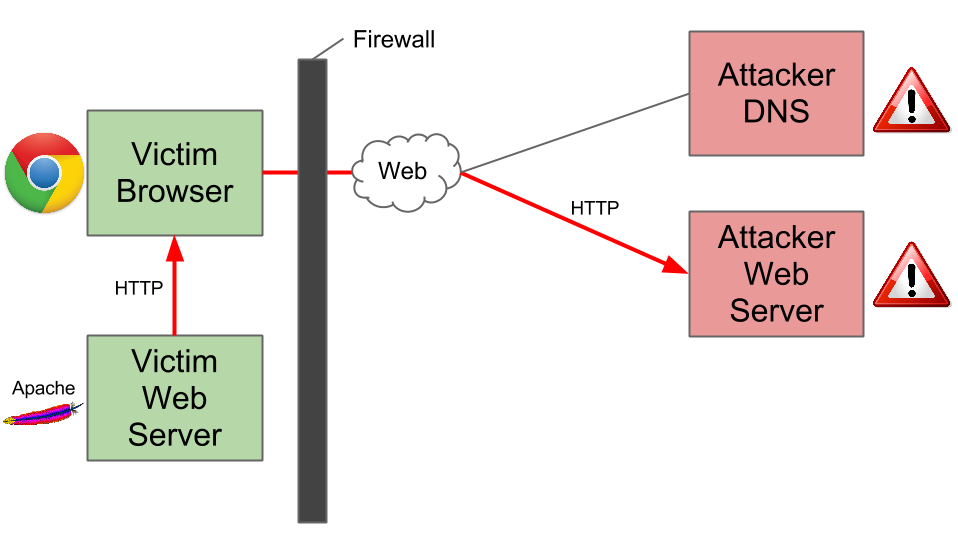
\includegraphics[width=0.8\columnwidth]{dnsrebind1.png}
\caption{\textbf{Traditional DNS Rebinding attack.} Once the victim's browser has established connection to both servers, it can relay data from the internal server back to the attacker's server.  The attacker can use this to gain access to private information stored on the victim's intranet.}
\label{fig:dnsrebind1}
\end{figure}


A common defense against the traditional attack is DNS pinning. With DNS pinning, the browser will cache the result of the DNS lookup for a period of time regardless of the response's TTL. This defense is not entirely effective though, as browser plug-ins generally maintain separate DNS entry databases. Such \emph{multi-pin} vulnerabilities are the result of each plug-in mapping to a different IP address, and then communicating with one another in order to execute the attack. However, many multi-pin vulnerabilities have been closed as well by the developers of the plug-ins. 

Our work focuses on executing a DNS rebinding attack by flooding the DNS cache used for DNS pinning on the victim's browser. We flood the cache with invalid entries in order to force the browser to do the vital second DNS lookup. In order to demonstate this exploit, we implement FireDrill, a tool that uses this vulnerability to initialize a fully interactive session between the attacker and the victim's web server.

The rest of the paper is organized as follows: Section 2 discusses related work on DNS rebinding. Section 3 introduces the cache flooding exploit and outlines our implementation of FireDrill. Section 4 evaluates this technique against alternative approaches. Section 5 discusses defenses and future work. Section 6 concludes.
         % 1.0 pg
\section{Related Work}
\label{sec:related}

%1pg

Jackson et al \cite{protectFromDNS} surveyed a number of previously undiscovered DNS rebinding attacks that exploit interactions between browsers and their plug-ins. Many of the attack vectors described in this paper have been closed since its publication. Their work outlines the possibility of using DNS rebinding not only for connecting to otherwise inaccessible services, but also for accessing public services using the victim's IP address. Once the attacker has hijacked the victim's IP address, he can execute a number of attacks including committing click fraud, sending spam, defeating IP-based authentication, and framing the victim. Each of these has important ramifications, but are all outside the scope of our work.

Other tools have been created which take different approaches to DNS rebinding, and have different intended uses. One tool, called Rebind \cite{rebind}, implements the multiple A record DNS rebinding attack. However, since the multiple A record attack is only possible when all the records are public IP addresses, this kind of attack cannot be used on local addresses. The author worked within this limitation, and made the target of the attack the victim's router's public IP address. This attack vector relies on exploiting default passwords on the router hardware, and the frequency with which the default credentials are left unchanged. Our approach does not require using only public IP addresses because at its root, our approach is not a multiple A record attack, it is a time-varying attack.  We are able to gain access to the entire intranet via binding to local IP addresses.

Byrne also demonstrated how to turn a victim's browser into a proxy using a standard time-varying and plug-in attack \cite{blackhat}. However, those attacks have their limitations: standard time-varying attacks potentially require several minutes to complete due to DNS pinning. Our approach accomplishes a similar result, while requiring a fraction of the time. The vulnerabilities that enable a plug-in attack have been mostly closed, and thus require the user to have an old version of a browser plug-in installed, such as Java or Flash Player. Such vulnerabilities have been patched out of most if not all modern versions of the plug-ins.

Finding web servers on the victim's intranet is a well-solved problem. It has been demonstrated by scanning IP addresses in JavaScript and monitoring responses\cite{grossman}, and various host-name-guessing techniques\cite{protectFromDNS}. Thus, it is not a focus of this work.


       % 1.0 pg
%\clearpage
\section{Implementation}
\label{sec:impl}



          % 1.5 pg
\section{Evaluation}
\label{sec:eval}
We measured our DNS rebinding attack by two primary factors. We analyzed the \emph{time to launch} and the \emph{impact} of the attack. We then compared it to other two DNS rebinding mechanisms. 

\subsection{Time to Launch}
To protect from a time-varying attack that is able to establish an interactive session between the malicious server and the broswer, most modern browers have implemented DNS pinning that pin a DNS record for a period of time. At this time, a time-varying attack would take ~160 seconds to launch according to our experiment on the latest Chrome browser. However, by flooding the DNS table, we found that in the current Chrome implementation, if a DNS record is kicked out from the cache, the pinning time would dramatically decrease. We found that in our attack, only ~10 seconds is needed to launch the attack on a browser that have 100 entries. 

In early 2013, the Chromium community has increased the size of DNS cache from 100 to 1000. This is not a really security patch but a performance related patch. We then ran our experiments on the staging version Chrome, and found that it would only take 10 more seconds to flood the DNS table and launch the attack. 

Another approach of DNS rebinding is based on multiple A records attack. This attack needs only a small amount of time due to the number of packets transmitted, however this attack has certain limitations, we will discuss it in the next subsection.

\subsection{Impact}
We now evaluate the impact of our attack against other DNS rebinding approaches. As mentioned in the last section, the multiple DNS record approach has the advantage of using less time to launch. However, it has several limitations on its impacts. 1) The rebinded IP address cannot be an internal IP address, otherwise the browser will priorize it and select it in the first place which results in a failure in DNS rebinding. 2) The attacker cannot change the rebinded IP address on the fly, which makes it unable to scan the subnet. 

For time-varying attack, although it is possible to bind to an internal IP address, it is also hard to change the rebinded IP address on the fly due to the extremly long launching time. 

In our experiement, we are able to use FireDrill to rebind the domain name to an internal IP address to build a interactive session. Also, we are able to dynamically change the IP address during an attack. The attacker has the ability to navigate through the entire subnet instead of just one single IP address.

\subsection{Making The Victim Stay}
Our attack needs the victim's browser to act as a proxy. Thus it requires the victim to stay in the page for the attacker 
          % 1.0 pg
\section{Discussion}
\label{sec:disc}

Many in the security community consider DNS rebinding attacks to be dead. However, we aimed to show in this work that there are ongoing developments in the area, and that DNS rebinding attacks are still possible on modern hardware and software configurations. Along with motivating further work on DNS rebinding, we hope to introduce some preliminary defenses against the particular techniques we proposed in this paper.

\subsection{Defense Against DNS Rebinding}

A significant amount of work has been done in the area to defend against DNS rebinding attacks at each stage of the process. Browsers, plug-ins, DNS resolvers, firewalls, and servers can all be augmented to help defend against the attack \cite{protectFromDNS}. Many of the most promising defenses have been implemented, such as DNS pinning and patching many of the plug-in vulnerabilities.

\subsection{Defense Against DNS Cache Flooding}

DNS cache flooding is a new method of forcing the second DNS lookup which is crucial to the success of a DNS rebinding attack. We demonstrated that it is possible to use this technique on modern browsers, but we believe a few simple provisions will be able to successfully defend against it. 

\begin{itemize}
\item \emph{Increase Cache Size.} Making the cache large enough that cache flooding takes prohibitively long is a very practical approach. However, it is not clear whether this will prevent this attack in its entirety, but rather make it impractical. There are also performance concerns involved with scaling up the DNS cache that should be taken into account before adopting this approach. 
\item \emph{Smarter Cache Eviction.} Cache flooding is made possible by the fact that invalid entries are being inserted into the table, which evict valid entries. The entries are invalid because the requests disobey same-origin policy, so an attempt resolve them should not occur. If the browser insists on inserting these invalid entries to the DNS cache, they should atleast be the first to be evicted when the cache is full.
\end{itemize}

\subsection{Future Work}

FireDrill brings together many existing and novel ideas in order to demonstrate a very powerful DNS rebinding attack. Ensuring that the malicious DNS, web server, attacker interface, and other pieces are working in unison is a complex task. Spending some time automating the process of launching these utilities and monitoring for potential victims could reveal some opportunities to improve the efficiency and impact of the attack as a whole.

Many of the original attack vectors of DNS rebinding achieved nearly instantaneous execution, but have since been closed and patched. At this point, we are able to achieve a DNS rebinding attack on modern browsers in ~10 seconds. While this is an improvement over alternative approaches, it can still be a prohibitively long duration to wait.  The defense strategy for DNS rebinding focuses on preventing the browser from doing a second DNS lookup. Exploring new ways of circumventing defenses could lead to a new, faster, form of the attack.

The impact of this and other DNS rebinding attacks could be expanded by examining the potential for using cookies during the attack. If a cookie could be used to authenticate as the victim when accessing either internal or external websites, the breadth of the attack could be amplified. Doing so would eliminate otherwise challenging steps such as using social engineering to gain access to authentication credentials.

XYZ-defenses




          % 0.5 pg
\section{Conclusions}
\label{sec:conc}

          % 0.25 pg

%Uncomment this line if your paper has / uses end notes
%\theendnotes

{%\footnotesize
\raggedright
\bibliographystyle{abbrv}
\bibliography{bib}
}

\end{document}

